\section{作业题目：结构力学基础与技巧班第2次作业（理论力学回顾）}
\begin{analysisbox}
支座反力题统一从整体隔离体入手，列水平力、竖向力和力矩平衡。若求得反力为负，说明真实方向与假设方向相反，数值仍可直接代入后续内力计算。
\end{analysisbox}
\subsection*{第 1 页转写}
求解图示结树的支性反力

30kN

15kN/m

3m

(a)

(b)

4kNm

40kN

0.2kN/m

30kN-m

10m

4m

(c)

(d)

20kNm20kN

6kN m

5a

3m

(e)

(f)

15kN.10kN.m

5kN/m

1m

2.5m

1m

2m

(5)

(h)

M.

2M.

3a

5a

3a

(1)
\begin{figure}[H]\centering
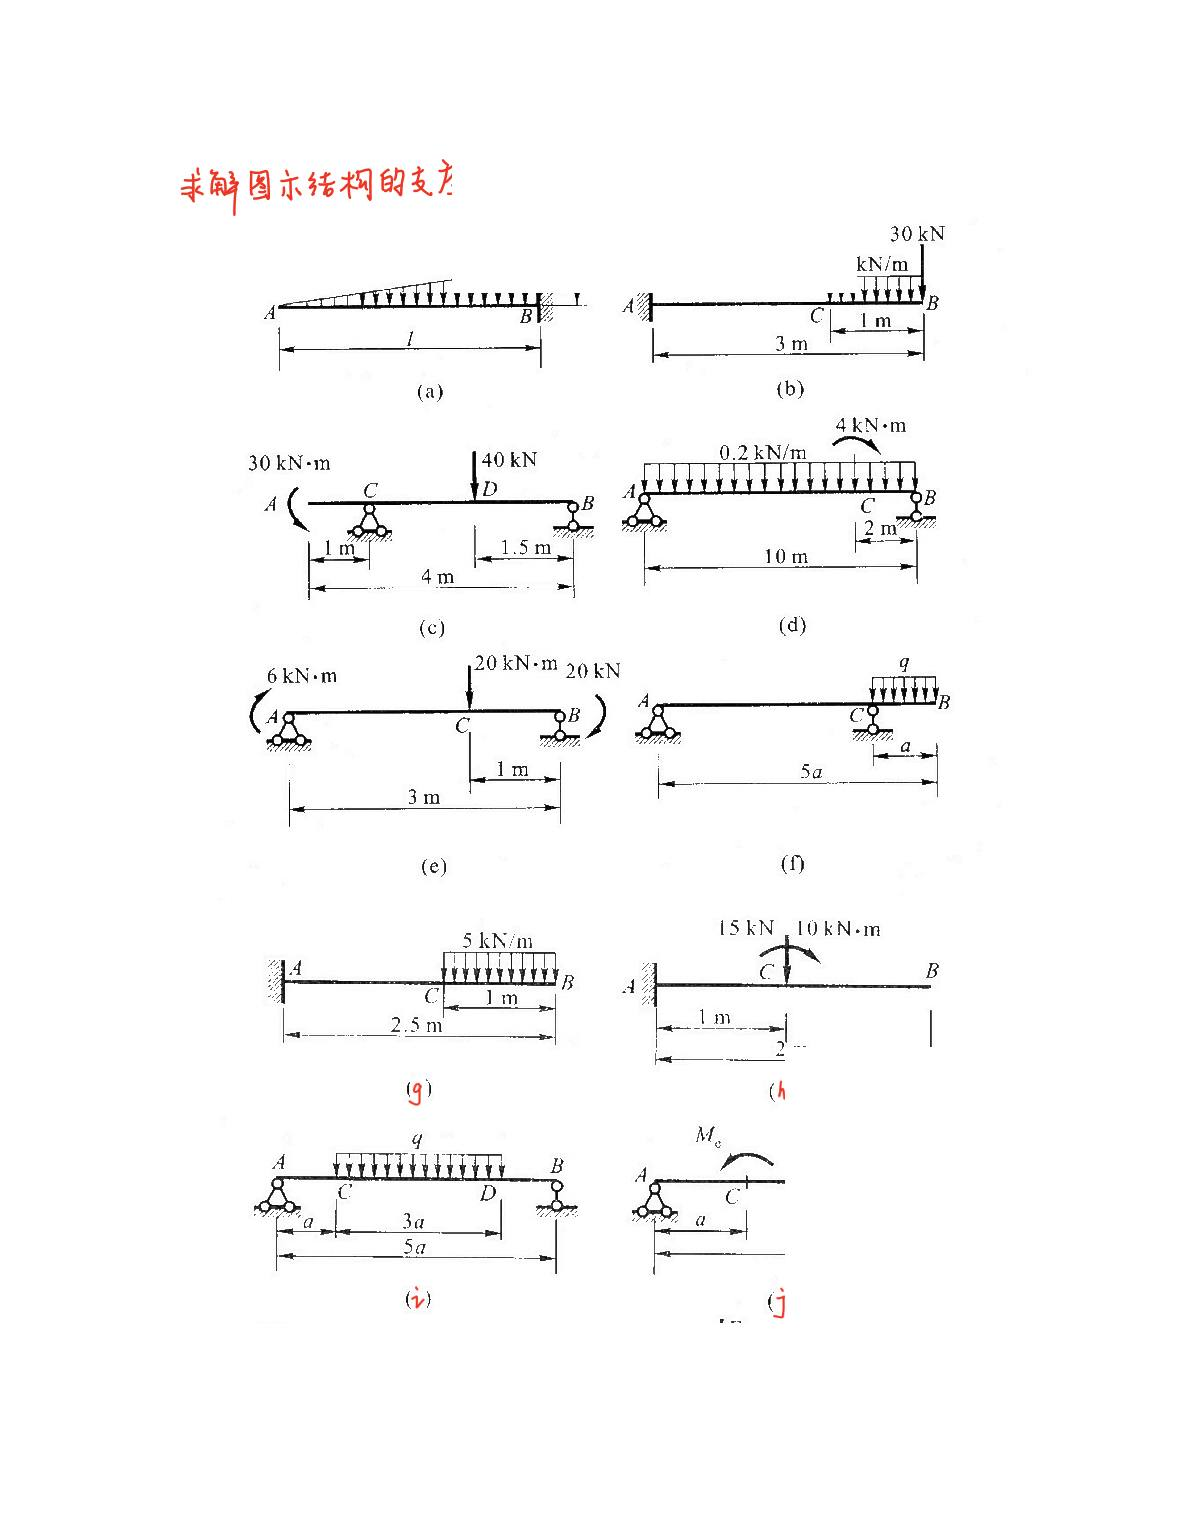
\includegraphics[width=0.92\textwidth]{figures/src04_p001.jpg}
\caption{结构力学基础与技巧班第2次作业（理论力学回顾） 第 1 页清理图形页}
\end{figure}
\subsection*{第 2 页转写}
5m

5m

()

(m)
\begin{figure}[H]\centering
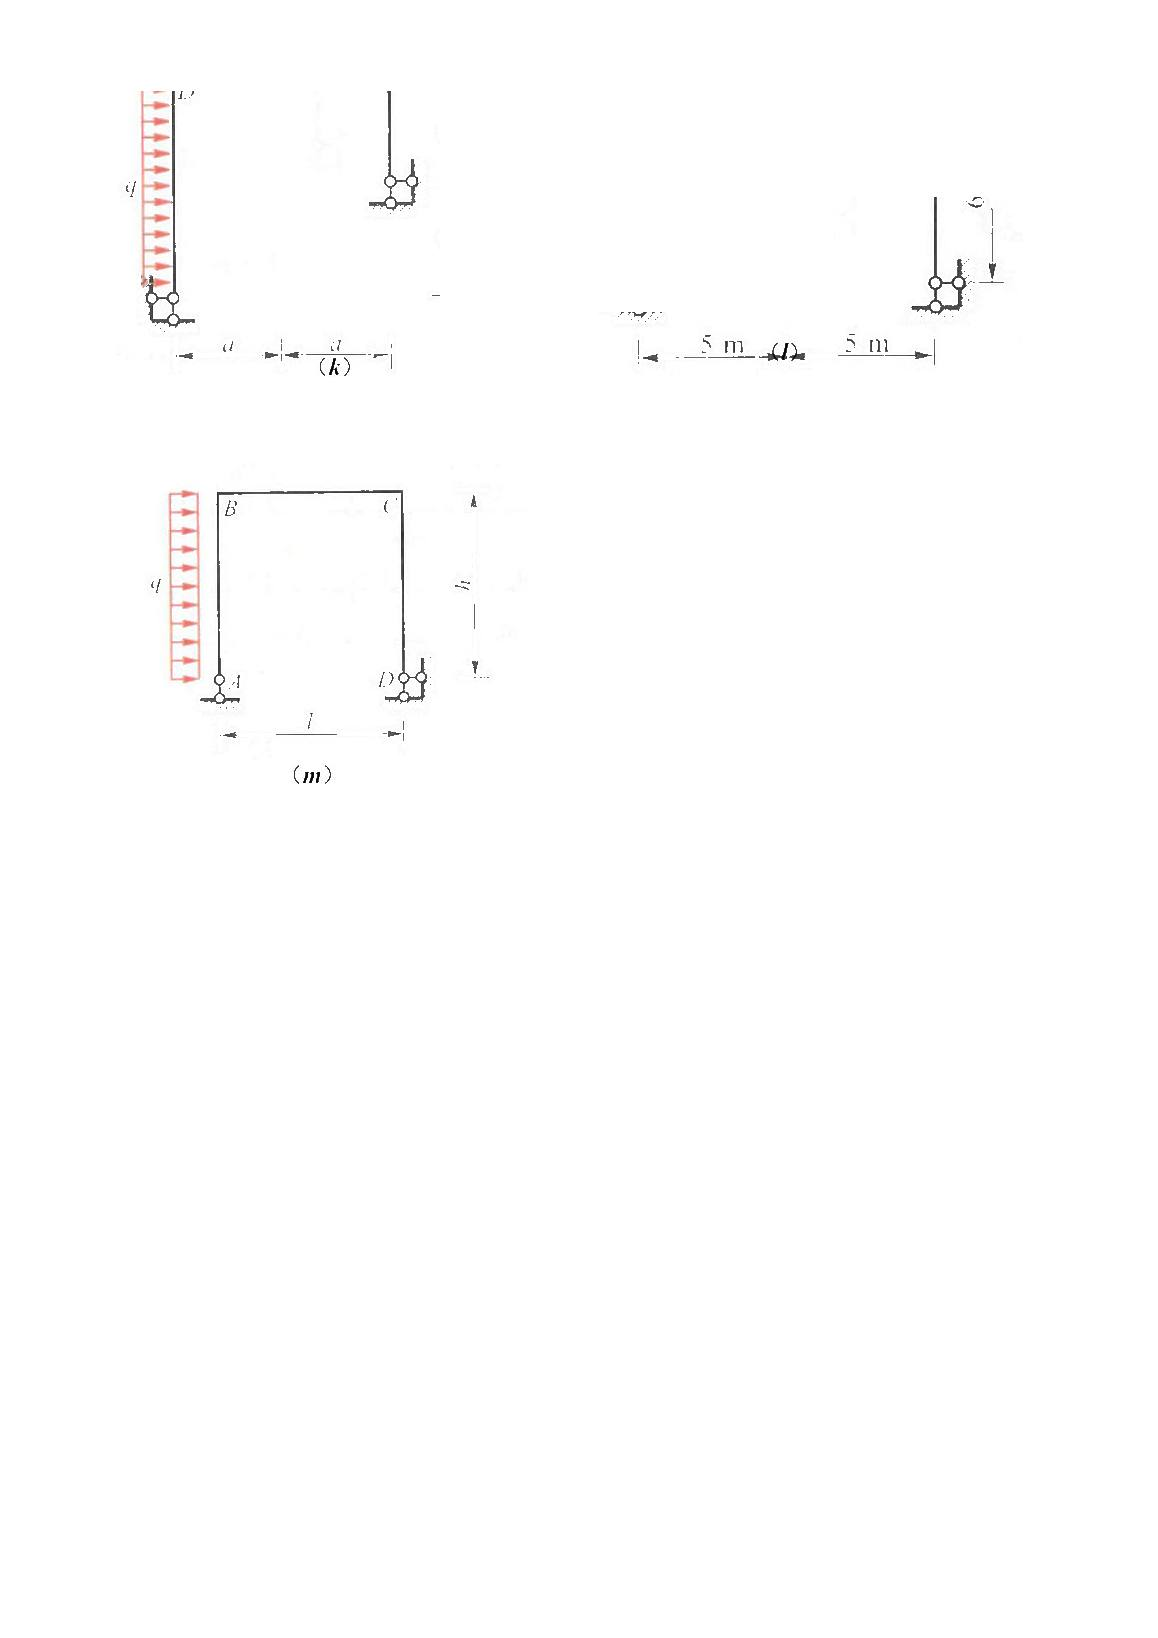
\includegraphics[width=0.92\textwidth]{figures/src04_p002.jpg}
\caption{结构力学基础与技巧班第2次作业（理论力学回顾） 第 2 页清理图形页}
\end{figure}
